\documentclass[10.5pt]{article}
\usepackage{amsmath,amsthm,amssymb}
\usepackage{mathtools}
\usepackage{enumerate}
\usepackage{graphicx}
\usepackage{mathpazo}
\usepackage{lmodern}
\usepackage{parskip}
\usepackage{fancyhdr}
\usepackage{wrapfig}
\usepackage{tikz}
\usepackage{hyperref}
\usetikzlibrary{positioning}
\usepackage[margin=1in]{geometry}
\newcommand{\jostle}{\texttt{Jostle}}
\lhead{Jacob Imola Research Proposal}
\rhead{}
\cfoot{\thepage}
\pagestyle{fancy}
\begin{document}
\centerline{\textbf{Automatic, Fine-Grained Algorithmic Choice for Differential Privacy}}
\centerline{Keywords: Statistical Disclosure, Differential Privacy, Private Algorithms, Dynamic Choice}
Releasing some information about a private database, or \emph{statistical disclosure}, is certainly beneficial for society --- for example, a  healthcare company allowing researchers to analyze their patient databases. However, such disclosures are fraught with accidental privacy leaks; the most famous example being Netflix \cite{Narayanan:2006}, and more recent examples being \href{https://hackernoon.com/how-to-rob-an-airbnb-252e7e7eda44}{AirBnB} and \href{https://gizmodo.com/this-is-almost-certainly-james-comey-s-twitter-account-1793843641}{Instagram}. As we move towards an increasingly data-driven future, privacy leaks become an immediate concern. Protecting against these leaks requires defining a notion of privacy and analyzing code to ensure that it meets the desired privacy level. However, most programmers are not privacy experts, and furthermore, analyzing large codebases is a tedious and error-prone process.

Many problems that place unneeded burden on programmers are dealt with via abstraction: for instance, object-oriented programming is a data abstraction that allows for efficient reuse of code. Therefore, it makes sense to make privacy abstract for the use case of privacy-naive programmers working with large code bases. For a programming language to adequately address this use case, it would need to not only abstract privacy but help the programmer select the right algorithm and parameters for the situation. Notable previous attempts build privacy-checking into either the static type system \cite{Reed:2010} or dynamic language constructs \cite{McSherry:2010}, preventing privacy by not compiling  or throwing runtime errors whenever they detect that too much privacy is being leaked. In either case, a privacy-naive programmer would gain no insight into whether they made a suboptimal algorithm choice which is breaking their code. This problem is noted by the authors of DPComp \cite{Hay:2016}, who comment that currently, ``the practitioner is lost and incapable of deploying the right algorithm''.

\begin{wrapfigure}{r}{0.33\textwidth}
\begin{center}
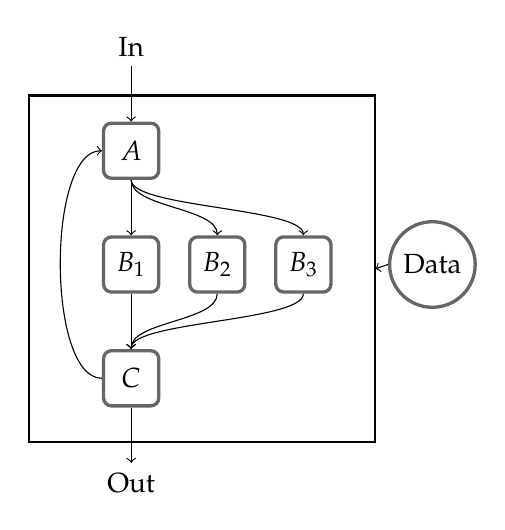
\begin{tikzpicture}[
squarednode/.style={rectangle, draw=black!60, very thick, minimum size=7mm, rounded corners=1mm},
roundnode/.style={circle, draw=black!60, very thick, minimum size=7mm}
]
\node[squarednode] (A) {$A$};
\node (In) [above=2em of A] {In};
\node[squarednode] (B1) [below=2em of A]{$B_1$};
\node[squarednode] (B2) [right=1em of B1]{$B_2$};
\node[squarednode] (B3) [right=1em of B2]{$B_3$};
\node[squarednode] (C)  [below=2em of B1]{$C$};
\node (Out) [below=2em of C] {Out};
\node[roundnode] (D) [right=2em of B3]{Data};
\draw[->] (A) -- (B1);
\draw[->] (A.south) .. controls+(down:1em) and +(up:1em) .. (B2.north);
\draw[->] (A.south) .. controls+(down:1em) and +(up:1em).. (B3.north);

\draw[->] (B1) -- (C);
\draw[->] (B2.south) ..controls+(down:1em) and +(up:1em) .. (C.north);
\draw[->] (B3.south) ..controls+(down:1em) and +(up:1em) .. (C.north);

\draw[->] (C.west) .. controls+(left:2em) and +(left:2em) .. (A.west);
\draw[thick] (-1.3,0.7) rectangle(3.1,-3.7);
\draw[->] (D.west) -- (3.1, -1.5);
\draw[->] (In) -- (A);
\draw[->] (C) -- (Out);
\end{tikzpicture}
\end{center}
\caption{An example algorithm that combines 3 subroutines $A$, $B$, and $C$. Subroutine $B$ can be accomplished in 3 different ways: $B_1$, $B_2$, and $B_3$.}
\label{fig:1}
\end{wrapfigure}
Together with my advisor, I plan to develop a programming language, \texttt{Jostle}, that will explore the fine-grained algorithmic choices automatically. In \texttt{Jostle}, the programmer represents their code as a network of subroutines for which the privacy and accuracy are known, some of which may solve the same problem yet may outperform one another depending on the data. \texttt{Jostle} will then explore the space of privacy and accuracy of these interchangeable subroutines during runtime to try to maximize privacy subject to each subroutine having certain accuracies. Figure \ref{fig:1} contains an algorithm with three subroutines. Subroutine $B$ could be accomplished in 3 different ways: $B_1$, $B_2$, and $B_3$. This is where \texttt{Jostle} could make an important runtime decision that would be superior to using just one of the $B_i$ separately: pick whichever $B_i$ has better privacy for the particular data and input parameters. The performance differences of the $B_i$ could be massive as demonstrated by DPComp \cite{Hay:2016}. For example, suppose that $B_1$ computes a private Support Vector Machine Classifier while $B_2$ computes a private Regularized Logistic Regression Classifier. Figure \ref{fig:2} shows slices of a privacy-accuracy-hyperparameter search space in which \texttt{Jostle} would optimize for a particular dataset. On the dataset, Logistic Regression tends to have better accuracy for a fixed privacy, but that may not always be the case. In general, the search space would consist of the amount of privacy, the amount of accuracy, and any input parameters to a subroutine. 

For the scope of this proposal, I plan to implement a runtime solution for exploring algorithmic choice. Faceted execution \cite{Austin:2013} is a good starting place because facets represent two separate, independent executions of a program. The two classifiers example will look like:
\begin{verbatim}
label a
    restrict a: accuracy(data, C) > 0.8
    let classifier = <a? Logistic(C) : SVM(C)>
\end{verbatim}

The \verb|label| command creates a new label that will make the decision of which function to use based on its restrictions. The \verb|restrict| command will add a restriction to a label, in this case forcing the classifier to have accuracy more than 0.8 subject to the data and to $C$. The programmer, who knows how to find the accuracy of his models, will implement the \verb|accuracy| function. In general, \verb|accuracy| will be a probabilistic proposition that must be satisfied. Computing the proposition will require ideas from probabilistic programming and sampling \cite{Sampson:2014} \cite{Kucera:2017} because we will need to either find a closed form or sample during runtime from the distribution over all data; sampling is faster but less accurate. Doing this precisely without too much of a runtime overhead will be a challenge. Also, input parameters will need to be optimized so the subroutine both satisfies the proposition and minimizes privacy. It will be hard to choose an optimization strategy; convex optimization could be useful here, but if the algorithms are very complicated, then I will likely resort to heuristics or SMT solvers. I will enjoy working on these problems because I have experience in probability bounds as well as in optimization. 

\begin{figure}
\begin{center}
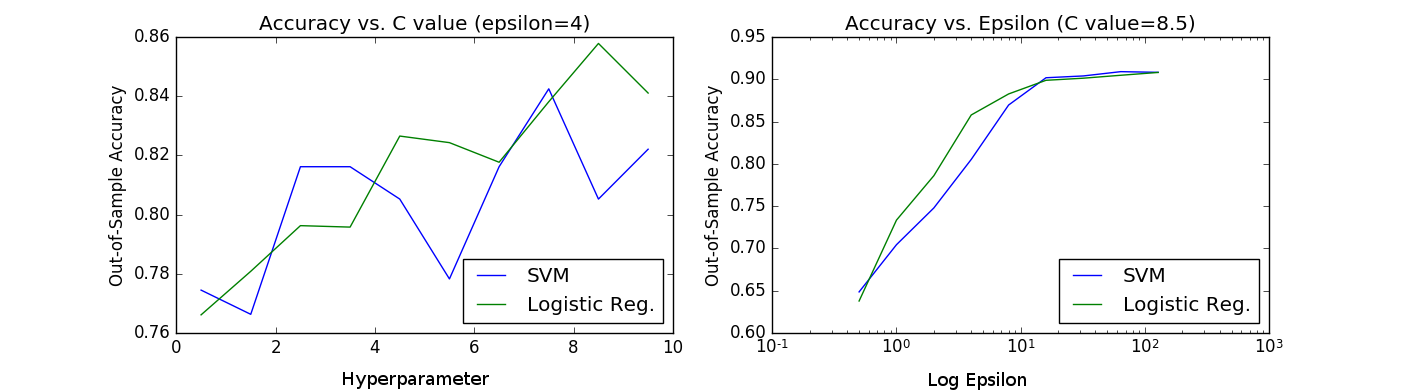
\includegraphics[scale=0.45]{PASS3.png}
\end{center}
\caption{The performances of two models, Support Vector Machines and Logistic Regression, trained on the famous \href{http://archive.ics.uci.edu/ml/datasets/Iris}{Iris} dataset. Above are two cross sections of the 3D space of the hyperparameter $C$, the differential privacy level $\epsilon$, and the out-of-sample accuracy in which \texttt{Jostle} would optimize.}
\label{fig:2}
\end{figure}
\textbf{Broader Impacts} \quad \texttt{Jostle} would be the first example of dynamically exploring execution paths to enforce privacy. It is a novel application of facets and probabilistic assertions and will provide more evidence of their usefulness. It will be the first time these language constructs have been used together. In addition, \texttt{Jostle} can be applied to optimize the usage of resources other than privacy such as processor and battery time. The extent to which \texttt{Jostle} is able to select an optimal algorithm will have enormous applications to artificial intelligence and to robotics. Finally, since \texttt{Jostle} abstracts privacy and removes the difficulty of selecting the proper algorithm, it will allow more programmers to write truly private code than ever before. It is my hope that \texttt{Jostle} will improve the privacy problems that affect our lives every day.

\bibliographystyle{plain}
{\footnotesize
\bibliography{Prospectus}}
\end{document}
